\documentclass[border=0.8ex,svgnames,tikz]{standalone}
\usepackage{amsmath,mathtools}
\usepackage{fontspec}
\setmainfont{Source Serif 4}
\setsansfont{Source Sans 3}
\setmonofont{Source Code Pro}
\usepackage{ifthen}
\usetikzlibrary{chains}
\newcommand{\ptrcolor}{LightSlateBlue}
\newcommand{\itcolor}{IndianRed}
\newcommand{\ritcolor}{LimeGreen}
\begin{document}
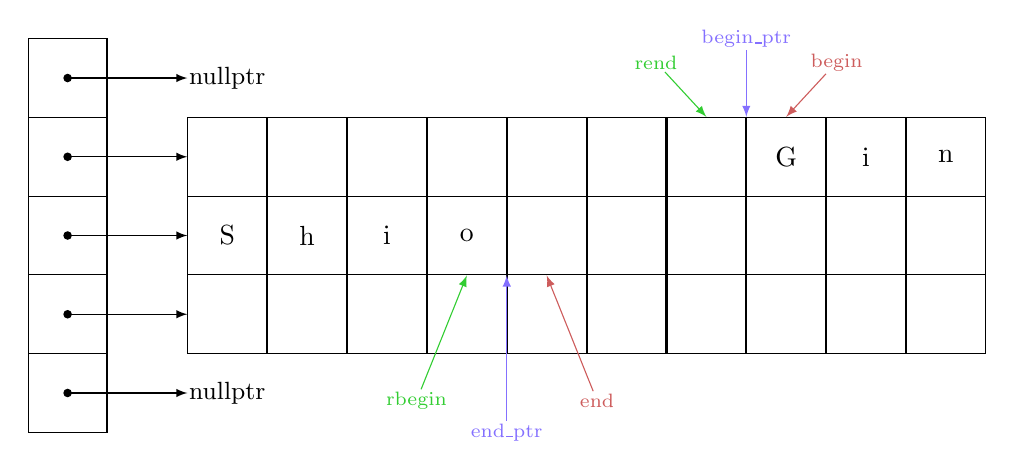
\begin{tikzpicture}
  \begin{scope}[
    node distance=0,
    every node/.style={draw,on chain,minimum width=1cm,minimum height=1cm},
    start chain=going right,
    ]
    \foreach \i in {0,...,4}{
      \coordinate(chunkin\i) at (0,\i);
      \chainin(chunkin\i);
      \node(chunk\i){};
      \path[fill](chunk\i) circle (0.36ex);
      \node[draw=none]{};
      \foreach \j in {0,...,9}{
        \ifthenelse{\i=0 \OR \i=4}{
          \node[draw=none](chunk\i\j){};
        }{
          \node(chunk\i\j){};
        }
      };
      \path[draw,>=latex] (chunk\i.center) edge[->] (chunk\i0);
    };
  \end{scope}
  \begin{scope}[
    every node/.style={minimum width=1cm,minimum height=1cm},
    every path/.style={draw,>=latex}
    ]
    \node[font=\small] at(chunk00) {nullptr};
    \node at(chunk37) {G};
    \node at(chunk38) {i};
    \node at(chunk39) {n};
    \node at(chunk20) {S};
    \node at(chunk21) {h};
    \node at(chunk22) {i};
    \node at(chunk23) {o};
    \node[font=\small] at(chunk40) {nullptr};
  \end{scope}
  \begin{scope}[
    every path/.style={draw,>=latex},
    every node/.style={draw=none,inner sep=0.2ex,font=\scriptsize},
    ]
    \path[color=\ptrcolor,text=\ptrcolor]
    (chunk37.west) ++(0,+1.5cm) node{begin\_ptr} edge[->] (chunk37.north west)
    (chunk24.west) ++(0,-2.5cm) node{end\_ptr} edge[->] (chunk24.south west);
    \path[color=\itcolor,text=\itcolor]
    (chunk37) ++(+0.64cm,+1.2cm) node{begin} edge[->] (chunk37.north)
    (chunk24) ++(+0.64cm,-2.1cm) node{end} edge[->] (chunk24.south);
    \path[color=\ritcolor,text=\ritcolor]
    (chunk36) ++(-0.64cm,+1.2cm) node{rend} edge[->] (chunk36.north)
    (chunk23) ++(-0.64cm,-2.1cm) node{rbegin} edge[->] (chunk23.south);
  \end{scope}
\end{tikzpicture}
\end{document}
